\documentclass[11pt]{article}

\usepackage{amsmath}
\usepackage{amssymb}
\usepackage{amsfonts}
\usepackage{amsthm}

\usepackage{graphicx}
\usepackage{tikz}
\usepackage{hyperref}
\usepackage{geometry}

\usepackage{bm}
\usepackage{mathtools}
\usepackage{enumitem}
\usepackage{cleveref}

\usepackage[numbers,sort&compress]{natbib}

\usetikzlibrary{arrows.meta,calc,positioning}

\geometry{margin=1in}
\hfuzz=8pt

\title{Gauge Freedom in Neural Representation Spaces}

\author{
Jericho Cain\\
Physics Department, Portland Community College, Portland, OR, USA\\
\texttt{jericho.cain@gmail.com}\\
ORCID: 0000-0003-4731-9142
}

\begin{document}
\hbadness=10000

\maketitle

\begin{abstract}

Neural network representations are typically analyzed as vectors in a fixed Euclidean space.
However, the coordinates of these vectors are not uniquely defined.
For any invertible linear transformation applied to the representation space,
the network function can be preserved by applying the inverse transformation
to downstream weights.
Consequently, representations are defined only up to invertible linear
transformations.
This paper develops a geometric framework that treats representation spaces
as vector spaces with a gauge freedom under the general linear group.
Within this framework, commonly used similarity measures such as cosine
similarity become metric-dependent quantities whose values can change under
coordinate transformations that leave the model function unchanged.
We show how several empirical observations in representation learning can be
interpreted through this lens.
In particular, previously reported instabilities of cosine similarity,
anisotropy in embedding spaces, and the motivation behind representation
comparison methods such as SVCCA and CKA arise naturally once this symmetry
is taken into account.
Finally, we demonstrate experimentally that inserting invertible linear
transformations inside trained networks can significantly alter cosine-based
representation geometry while leaving model predictions unchanged.
These results suggest that meaningful analysis of neural representations
should focus on geometric quantities that are invariant under the gauge
freedom of representation space.

\end{abstract}

\section{Introduction}

Modern neural networks operate by transforming inputs into sequences of
high-dimensional vector representations.
These representations appear throughout machine learning systems, including
word embeddings, hidden states in transformer models, and latent variables
in autoencoders.
Because of this ubiquity, a large body of work attempts to understand neural
models by analyzing the geometry of these vector representations.

A common assumption in such analyses is that the coordinates of the
representation vectors carry intrinsic geometric meaning.
Similarity between representations is frequently measured using cosine
similarity or Euclidean distance, and structural properties of the
representation space are studied through principal components, clustering,
or subspace comparisons.

However, the coordinates of neural representations are not uniquely defined.
Consider a hidden representation

\[
h(x) \in V, \qquad V = \mathbb{R}^d .
\]

For any invertible matrix $D \in GL(d)$ we may transform the representation as

\[
\tilde h(x) = D h(x).
\]

If the weights of the subsequent layer are transformed accordingly,
the overall function computed by the network remains unchanged.
Thus two representation systems related by an invertible linear
transformation encode the same information even though the coordinates
of the vectors differ.

This observation implies that representation spaces possess a symmetry under
invertible linear transformations.
From a geometric perspective, the representation vectors are therefore
defined only up to a change of basis.
We refer to this freedom as a gauge symmetry of representation space.

Once this symmetry is taken into account, several empirical observations in
representation learning become easier to interpret.
For example, cosine similarity is often used to measure semantic similarity
between embeddings.
However, cosine similarity depends on the metric structure of the space.
Under a linear transformation $h \mapsto Dh$, cosine similarity between
representations generally changes even though the encoded information
remains the same.

Recent work has reported related phenomena in several contexts.
Steck et al.~\cite{Steck2024} show that cosine similarity applied to learned
embeddings in matrix factorization models can yield arbitrary results due
to scaling freedoms in the factorization.
Ai~\cite{Ai2026} argues that cosine similarity captures only angular
relationships between vectors and may fail to reflect other meaningful
relations in embedding spaces.
Meanwhile, representation comparison methods such as SVCCA and CKA have been
proposed to compare neural representations while remaining insensitive to
certain linear transformations.

In this paper we develop a geometric framework that places these observations
into a common perspective.
We treat neural representations as elements of a vector space defined only
up to invertible linear transformations and examine the consequences of this
symmetry for representation analysis.

Our contributions are threefold.

First, we formalize the gauge freedom of representation space and show how
common similarity measures depend on implicit metric assumptions.

Second, we interpret several empirical phenomena in representation learning,
including anisotropy, feature superposition, and intrinsic dimensionality,
within this geometric framework.

Third, we demonstrate experimentally that inserting invertible linear
transformations inside trained networks can significantly alter cosine-based
representation geometry while leaving model predictions unchanged.

Together these results suggest that analyses of neural representations should
focus on geometric quantities that are invariant under the gauge symmetry of
representation space.

\section{Representation Spaces}

Neural networks transform inputs into intermediate vector representations.
These representations appear as hidden states in feedforward networks,
transformer activations, or latent variables in autoencoders.
Understanding the structure of these representations is central to many
approaches for interpreting neural models.

Let $\mathcal{X}$ denote the input space and let a neural network define a
mapping

\[
f_\theta : \mathcal{X} \rightarrow \mathcal{Y},
\]

parameterized by weights $\theta \in \mathbb{R}^p$.

At an intermediate layer $\ell$, the network produces a hidden
representation

\[
h_\ell(x;\theta) \in V,
\]

where $V = \mathbb{R}^d$ is a $d$-dimensional vector space.
We refer to $V$ as the \emph{representation space} of layer $\ell$.

For a dataset $\{x_i\}_{i=1}^n$, the representations produced by the
network form a collection of vectors

\[
h_\ell(x_1;\theta),\dots,h_\ell(x_n;\theta) \in V.
\]

These vectors can be arranged into a representation matrix

\[
H =
\begin{pmatrix}
h_\ell(x_1;\theta) & \cdots & h_\ell(x_n;\theta)
\end{pmatrix}
\in \mathbb{R}^{d \times n}.
\]

Many empirical analyses of neural networks examine the geometry of these
representations.
Examples include similarity comparisons between embeddings, clustering
structure in hidden states, and dimensionality reduction techniques such
as principal component analysis.

Throughout this work we treat the representation space $V$ as a vector
space equipped with an inner product

\[
\langle u,v\rangle = u^\top v.
\]

This inner product induces the Euclidean metric

\[
\|u\| = \sqrt{u^\top u}.
\]

Common similarity measures such as cosine similarity are defined with
respect to this metric.
However, as we show in the next section, the coordinates of representation
vectors are not uniquely defined.

\section{Gauge Freedom of Representations}

The coordinates of neural representations are not uniquely defined.
To see this, consider a representation

\[
h(x) \in V = \mathbb{R}^d.
\]

Let $D \in GL(d)$ be any invertible matrix.
Define a transformed representation

\[
\tilde h(x) = D h(x).
\]

If the next layer of the network computes

\[
y = W h(x),
\]

then after the transformation we may write

\[
y = W D^{-1} \tilde h(x).
\]

Thus the same network function can be expressed using the transformed
representation $\tilde h$ provided the downstream weights are adjusted
accordingly.

Consequently, two representation systems related by an invertible linear
transformation

\[
h(x) \mapsto D h(x)
\]

encode identical information for the purposes of the network computation.

This observation implies that representation spaces possess a symmetry
under invertible linear transformations.
In other words, the vectors $h(x)$ are defined only up to a change of
basis in the representation space $V$.

We refer to this symmetry as a \emph{gauge freedom} of representation space.
Formally, the representation vectors are defined modulo the action of the
general linear group

\[
GL(d).
\]

While this freedom does not affect the function computed by the network,
it can alter geometric properties of the representation coordinates.
In particular, quantities that depend on the metric structure of the
space—such as cosine similarity—may change under such transformations.

Understanding which properties of representations remain invariant under
this symmetry is therefore essential when analyzing neural representation
geometry.

\section{Metric Structure and Similarity Measures}

The gauge freedom described in the previous section implies that the
coordinates of representation vectors are not uniquely defined.
Consequently, geometric quantities that depend on the metric structure
of the representation space may vary under invertible linear
transformations.

Let $u,v \in V$ be two representation vectors.
Cosine similarity is commonly used to measure their similarity:

\[
\cos(u,v) =
\frac{u^\top v}{\|u\|\|v\|}.
\]

This quantity implicitly assumes the Euclidean metric on $V$.

Now consider a gauge transformation

\[
\tilde u = D u,
\qquad
\tilde v = D v,
\]

where $D \in GL(d)$.
The inner product between the transformed vectors becomes

\[
\langle \tilde u,\tilde v\rangle
=
u^\top D^\top D v .
\]

Thus the transformation induces a new inner product

\begin{equation}
\langle u,v\rangle_D
=
u^\top G v,
\qquad
G = D^\top D .
\label{eq:metric_pullback}
\end{equation}

Geometrically, the matrix $G$ acts as a metric tensor on the
representation space.
Under this metric, cosine similarity becomes

\[
\cos_D(u,v)
=
\frac{u^\top G v}
{\sqrt{u^\top G u}\sqrt{v^\top G v}}.
\]

Therefore cosine similarity is not invariant under general gauge
transformations of the representation space. Figure~\ref{fig:metric-distortion-ellipse} illustrates how a linear
distortion of the representation space changes angular relationships
between vectors by inducing a new metric tensor.
Two embedding systems related by an invertible linear transformation may
represent the same information while producing different cosine
similarity values.


\begin{figure}[htbp]
\centering
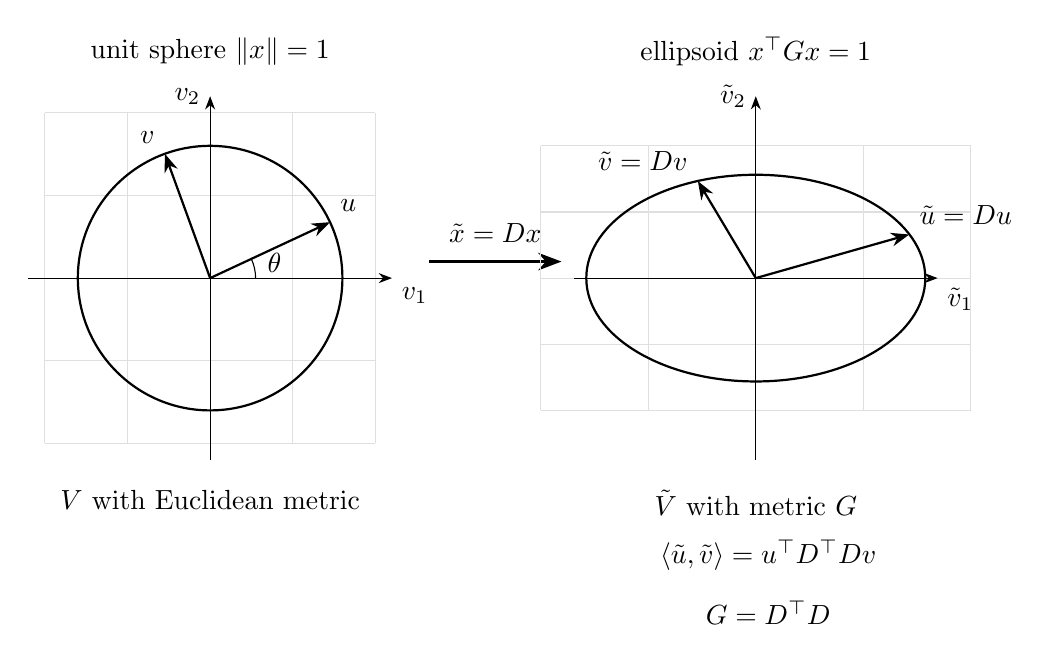
\begin{tikzpicture}[scale=1.05, >=Stealth]

  %-------------------------
  % Left panel: original space
  %-------------------------
  \begin{scope}

    % faint grid
    \draw[gray!25, thin] (-2,-2) grid (2,2);

    % Axes
    \draw[->] (-2.2,0) -- (2.2,0) node[below right] {$v_1$};
    \draw[->] (0,-2.2) -- (0,2.2) node[left] {$v_2$};

    % Unit circle
    \draw[thick] (0,0) circle (1.6);

    % Vectors
    \coordinate (O) at (0,0);
    \coordinate (u) at ({1.6*cos(25)},{1.6*sin(25)});
    \coordinate (v) at ({1.6*cos(110)},{1.6*sin(110)});

    \draw[thick,->] (O) -- (u) node[above right] {$u$};
    \draw[thick,->] (O) -- (v) node[above left] {$v$};

    % Angle marker
    \draw (0.55,0) arc (0:25:0.55);
    \node at (0.78,0.18) {$\theta$};

    % Labels
    \node[below] at (0,-2.45) {$V$ with Euclidean metric};
    \node[above] at (0,2.45) {unit sphere $\|x\|=1$};

  \end{scope}

  % Arrow between panels
  \draw[very thick,->] (2.65,0.2) -- (4.25,0.2);
  \node at (3.45,0.55) {$\tilde{x}=Dx$};

  %-------------------------
  % Right panel: distorted space
  %-------------------------
  \begin{scope}[xshift=6.6cm]

    % faint grid (slightly stretched visually to hint distortion)
    \draw[gray!25, thin, xscale=1.3, yscale=0.8] (-2,-2) grid (2,2);

    % Axes
    \draw[->] (-2.2,0) -- (2.2,0) node[below right] {$\tilde v_1$};
    \draw[->] (0,-2.2) -- (0,2.2) node[left] {$\tilde v_2$};

    % Ellipsoid
    \draw[thick] (0,0) ellipse (2.05 and 1.25);

    % Transformed vectors
    \coordinate (Ou) at (0,0);
    \coordinate (tu) at ({1.28*1.6*cos(25)},{0.78*1.6*sin(25)});
    \coordinate (tv) at ({1.28*1.6*cos(110)},{0.78*1.6*sin(110)});

    \draw[thick,->] (Ou) -- (tu) node[above right] {$\tilde u=Du$};
    \draw[thick,->] (Ou) -- (tv) node[above left] {$\tilde v=Dv$};

    % Geometry labels
    \node[above] at (0,2.45) {ellipsoid $x^\top G x = 1$};
    \node[below] at (0,-2.45) {$\tilde V$ with metric $G$};

    % Metric annotation
    \node[align=left] at (0.15,-3.35) {$\langle \tilde u,\tilde v\rangle
      = u^\top D^\top D v$};
    \node[align=left] at (0.15,-4.05) {$G=D^\top D$};

  \end{scope}

\end{tikzpicture}
\caption{A linear distortion $\tilde x = D x$ maps the Euclidean unit sphere to an ellipsoid. The induced inner product is $G=D^\top D$, so cosine similarity computed after the transformation corresponds to angular similarity in the distorted metric.}
\label{fig:metric-distortion-ellipse}
\end{figure}

\subsection{Whitening as a Canonical Gauge}

A particularly important case arises when the transformation removes
anisotropy in the representation distribution.

Let $\Sigma$ denote the covariance matrix of hidden states,

\[
\Sigma = \mathbb{E}[h h^\top].
\]

Defining the whitening transformation

\[
D = \Sigma^{-1/2}
\]

maps the covariance to the identity matrix.
In the transformed coordinates

\[
\tilde h = D h
\]

the representation distribution becomes isotropic,

\[
\mathbb{E}[\tilde h \tilde h^\top] = I.
\]

In these coordinates, cosine similarity corresponds to angular similarity
in a space where the representation distribution has unit covariance.
Equivalently, cosine similarity in the original coordinates can be
interpreted as angular similarity under the Mahalanobis metric induced by
$\Sigma$.

From the perspective developed here, whitening can therefore be viewed as
a choice of gauge that fixes the metric structure of the representation
space.

\subsection{Implications for Embedding Similarity}

Recent empirical work has observed that cosine similarity can behave
unexpectedly in embedding spaces.

Steck et al.~\cite{Steck2024} analyze cosine similarity in matrix
factorization models and show that the learned embeddings may contain
scaling freedoms that allow arbitrary rescaling of latent dimensions.
These rescalings leave the model predictions unchanged while producing
different cosine similarity values between embeddings.

Similarly, Ai~\cite{Ai2026} argues that cosine similarity captures only
angular alignment between vectors and may fail to reflect other
relationships between embeddings.

Within the geometric framework developed here, these observations arise
naturally.
Invertible linear transformations alter the metric structure of the
representation space while preserving the underlying information encoded
by the representations.
Similarity measures that depend on the metric, such as cosine similarity,
therefore become coordinate dependent.

This perspective suggests that analyses of neural representations should
focus on geometric properties that remain invariant under the gauge
freedom of representation space.

\section{Feature Directions and Subspaces}

Many analyses of neural representations attempt to identify interpretable
features encoded within hidden states.  These features are often modeled as
directions in the representation space.

Let $h(x) \in V = \mathbb{R}^d$ denote the representation of an input $x$.
Suppose that the representation can be approximated as a linear combination
of feature vectors,

\[
h(x) \approx F a(x),
\]

where

\[
F =
\begin{pmatrix}
f_1 & f_2 & \cdots & f_k
\end{pmatrix}
\in \mathbb{R}^{d \times k}
\]

is a matrix whose columns correspond to feature directions and
$a(x) \in \mathbb{R}^k$ are feature activations.

In this view, each feature corresponds to a direction in representation
space, and the representation vector encodes the strengths with which
these features are activated.

\subsection{Feature Packing and Superposition}

In many neural networks the number of potential features exceeds the
dimension of the representation space.
Consequently, multiple features may be encoded within overlapping
subspaces of the representation space.

This phenomenon is often described as \emph{feature superposition}.
In the linear model above, superposition occurs when the feature matrix
$F$ has more columns than the ambient dimension of the representation
space.

The geometry of feature interactions can be characterized by the
Gram matrix of the feature directions,

\[
G_F = F^\top F .
\]

When the columns of $F$ are orthogonal, the Gram matrix is diagonal and
features can be read out independently.
When the columns are not orthogonal, feature activations interact through
the off-diagonal entries of $G_F$, producing interference between
features.

This perspective highlights that feature superposition is fundamentally a
geometric property of the representation space rather than a property of
individual neurons.

\subsection{Gauge Transformations of Feature Bases}

Under a gauge transformation of the representation space,

\[
h \mapsto D h,
\qquad
D \in GL(d),
\]

the feature matrix transforms as

\[
F \mapsto D F .
\]

The Gram matrix of the features becomes

\[
F^\top F
\mapsto
F^\top D^\top D F .
\]

Thus the pairwise angles between feature directions depend on the metric
structure induced by the gauge choice.
Two representation systems related by an invertible linear transformation
may therefore contain identical information while exhibiting different
apparent feature geometries.

This observation again emphasizes that many geometric properties of
representations depend on the coordinate system used to describe the
representation space.

\subsection{Representation Similarity Across Networks}

A related problem arises when comparing representations produced by
different neural networks.
Given two representation matrices

\[
H_1 , H_2 \in \mathbb{R}^{d \times n},
\]

direct comparison of their coordinates is generally not meaningful
because the two representation spaces may differ by an invertible linear
transformation.

Several methods have been proposed to address this issue.
Canonical correlation analysis (CCA) and its variants align
representations by searching for linear projections that maximize
correlation between corresponding activations.
More recently, centered kernel alignment (CKA) compares representations
using Gram matrices of example similarities.

Within the geometric framework developed in this paper, such methods can
be interpreted as attempts to construct similarity measures that are less
sensitive to coordinate transformations of the representation space.

This interpretation suggests that meaningful comparisons between
representation spaces should focus on quantities that remain stable under
the gauge freedom described in Section~3.

\section{Representation Dynamics and Local Geometry}

The previous sections focused on the geometric structure of representation
spaces at a fixed set of network parameters.
During training, however, representations evolve as the parameters of the
network are updated.
Understanding how parameter updates affect representations provides a
useful perspective on the dynamics of learning.

Let $\theta \in \mathbb{R}^p$ denote the parameters of a neural network and
consider the representation at layer $\ell$

\[
h_\ell(x;\theta) \in \mathbb{R}^d .
\]

For small parameter changes $\delta \theta$, the corresponding change in the
representation can be approximated using a first-order Taylor expansion,

\begin{equation}
\delta h_\ell(x)
\approx
J_\ell(x) \, \delta \theta ,
\label{eq:linear_rep_dynamics}
\end{equation}

where

\[
J_\ell(x)
=
\frac{\partial h_\ell(x;\theta)}{\partial \theta}
\in \mathbb{R}^{d \times p}
\]

is the Jacobian of the representation with respect to the model parameters.

\subsection{Induced Metric on Parameter Space}

Equation~(\ref{eq:linear_rep_dynamics}) relates parameter updates to
representation changes.
Using the Euclidean norm in representation space, the squared magnitude of
the representation change becomes

\begin{equation}
\|\delta h_\ell(x)\|^2
\approx
\delta\theta^\top (J_\ell^\top J_\ell)\, \delta\theta .
\label{eq:rep_change_metric}
\end{equation}

The matrix

\[
G_\ell = J_\ell^\top J_\ell
\]

defines a positive semidefinite quadratic form on parameter space.
Geometrically, this matrix acts as a metric tensor describing how changes
in parameters affect the representation at layer $\ell$.

This construction is closely related to the idea of pullback metrics in
differential geometry.
The Jacobian maps directions in parameter space to directions in
representation space, and the metric $G_\ell$ measures parameter changes in
terms of the resulting change in representations.

\subsection{Interpretation for Training Dynamics}

The metric $G_\ell$ provides a local description of how sensitive the
representation is to parameter updates.
Directions in parameter space corresponding to large eigenvalues of
$G_\ell$ produce large changes in the representation, while directions
corresponding to small eigenvalues produce little change.

This perspective connects representation geometry to optimization.
Gradient-based learning updates parameters in directions determined by the
loss function, but the resulting change in the representation depends on
how these parameter directions are mapped through the Jacobian of the
network.

Consequently, different layers may experience different effective
geometries during training depending on the structure of their Jacobians.

\subsection{Gauge Dependence}

As in earlier sections, representation geometry depends on the coordinate
system used to describe the representation space.
Under a gauge transformation

\[
h_\ell \mapsto D h_\ell ,
\]

the Jacobian transforms as

\[
J_\ell \mapsto D J_\ell .
\]

The induced metric therefore becomes

\[
G_\ell \mapsto J_\ell^\top D^\top D J_\ell .
\]

Thus the local geometry describing representation dynamics depends on the
metric structure chosen for the representation space.
However, the functional behavior of the network remains unchanged under
such transformations, reflecting again the gauge freedom described in
Section~3.

\section{Empirical Demonstration of Gauge Freedom}

We provide a minimal empirical demonstration using a two-layer MLP trained
on the scikit-learn digits dataset.  Let

\[
h(x)=\mathrm{ReLU}(W_1 x+b_1), \qquad y(x)=W_2 h(x)+b_2 .
\]

After training, we sample an invertible matrix $D \in GL(d)$ and build an
equivalent network by inserting $D$ into representation space:

\[
\tilde h(x)=D h(x), \qquad \tilde W_2 = W_2 D^{-1},
\]

so that
\[
\tilde y(x)=\tilde W_2 \tilde h(x)+b_2 = W_2 h(x)+b_2 = y(x).
\]

In our run, the maximum absolute difference in logits between the original
and transformed networks was $1.48\times 10^{-5}$, with identical predicted
classes on the full test set.  This confirms functional invariance under
the gauge transformation.

We then computed pairwise cosine similarity matrices for hidden
representations before and after the gauge transform.  Although model
predictions were unchanged, cosine geometry shifted substantially:
the mean absolute cosine change over pairwise comparisons was
approximately $0.13$.

\begin{figure}[htbp]
\centering
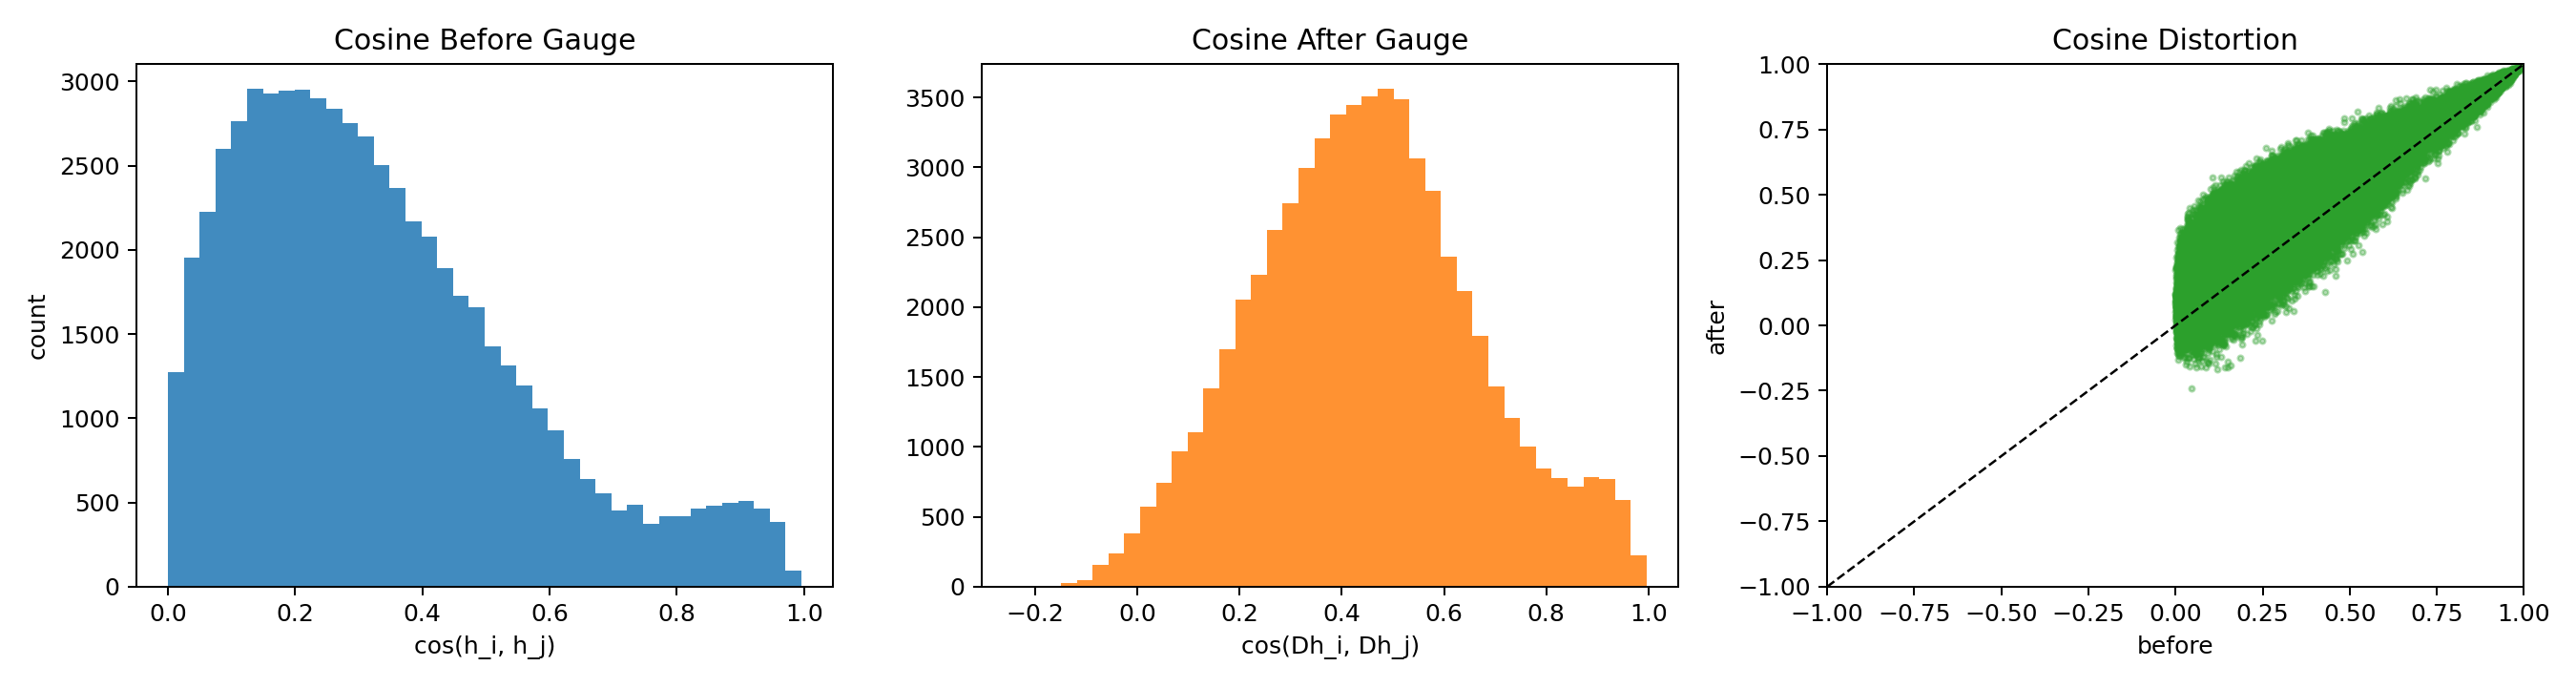
\includegraphics[width=\textwidth]{../experiments/figures/fig_cosine_distortion.png}
\caption{Gauge transformation leaves model outputs invariant but distorts
cosine geometry in representation space. Left: cosine distribution before
transform. Middle: after transform. Right: pairwise cosine values before
versus after transformation.}
\label{fig:cosine-distortion-empirical}
\end{figure}

\subsection{Nearest-Neighbor Instability and CIFAR-10 Corroboration}

To quantify a practical consequence of gauge dependence, we measured
nearest-neighbor instability under cosine similarity.
For each test embedding, we computed its top-$k$ cosine neighbors before
and after the gauge transform and evaluated mean Jaccard overlap.

On Digits (same MLP setting), the mean Jaccard overlap at $k=10$ was
approximately $0.721$, showing that local similarity rankings change
substantially even when model predictions are unchanged.

\begin{figure}[htbp]
\centering
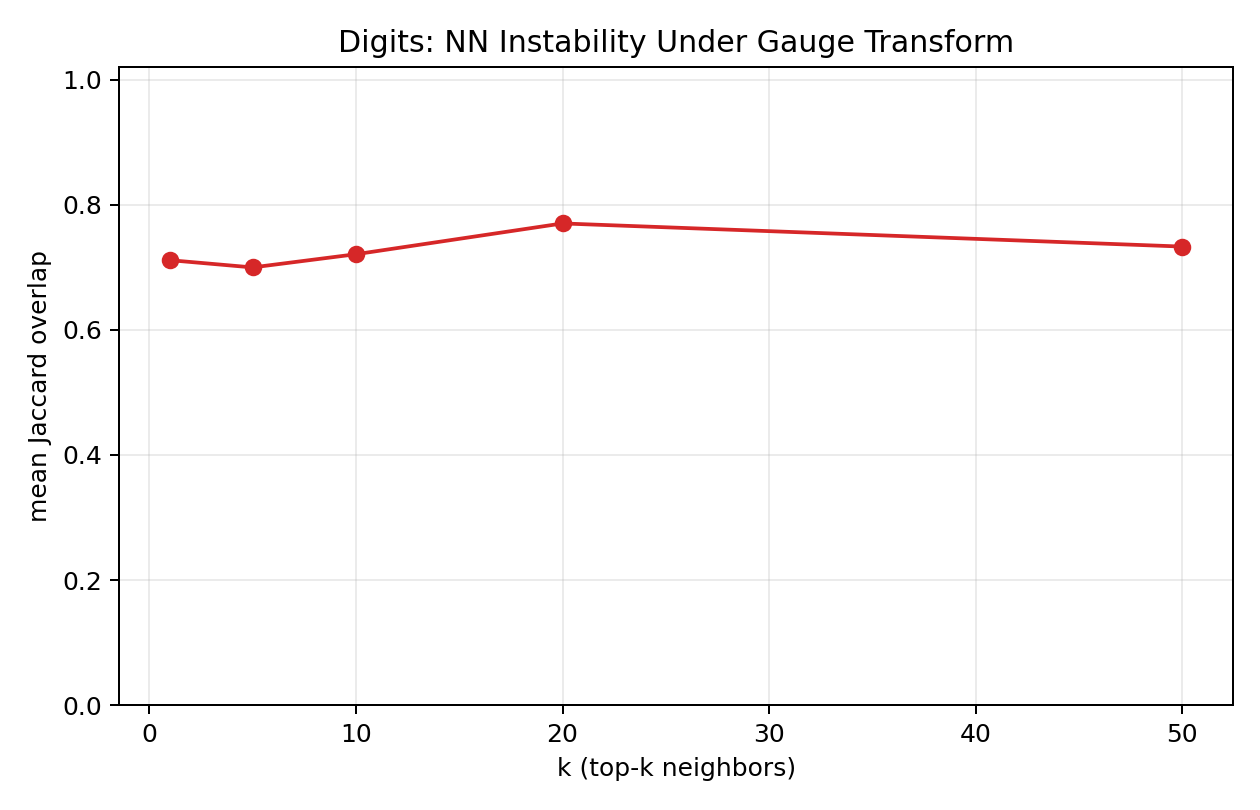
\includegraphics[width=0.75\textwidth]{../experiments/figures/fig_nn_instability_digits.png}
\caption{Digits nearest-neighbor instability under gauge transformation.
Mean Jaccard overlap between top-$k$ cosine neighbors before and after
transform remains significantly below $1$, despite functional invariance.}
\label{fig:nn-instability-digits}
\end{figure}

We then replicated the same gauge-invariance and geometry-distortion
analysis on CIFAR-10 using a small CNN and penultimate-layer features.
In this setting, test accuracy was approximately $0.682$ (5 epochs),
maximum logit difference after gauge compensation was
$1.34\times 10^{-5}$, prediction agreement was $1.0$, and mean absolute
cosine change was approximately $0.050$.
Nearest-neighbor overlap at $k=10$ was approximately $0.723$.

To make gauge strength explicit, we additionally swept a controlled family
of transforms with condition number $\kappa$.
For
\[
D(\kappa)=Q_1\operatorname{diag}(s_1,\ldots,s_d)Q_2,\qquad s_1/s_d=\kappa,
\]
cosine distortion increased and neighborhood stability decreased as
$\kappa$ increased.
For example, in our run:
\[
\kappa=1 \Rightarrow \text{mean }|\Delta\cos| \approx 0,\ \text{Jaccard@10}\approx 1,
\]
\[
\kappa=20 \Rightarrow \text{mean }|\Delta\cos| \approx 0.081,\ \text{Jaccard@10}\approx 0.629.
\]
Across the sweep, prediction agreement remained $1.0$ and logit
differences remained at numerical precision scale.

\begin{figure}[htbp]
\centering
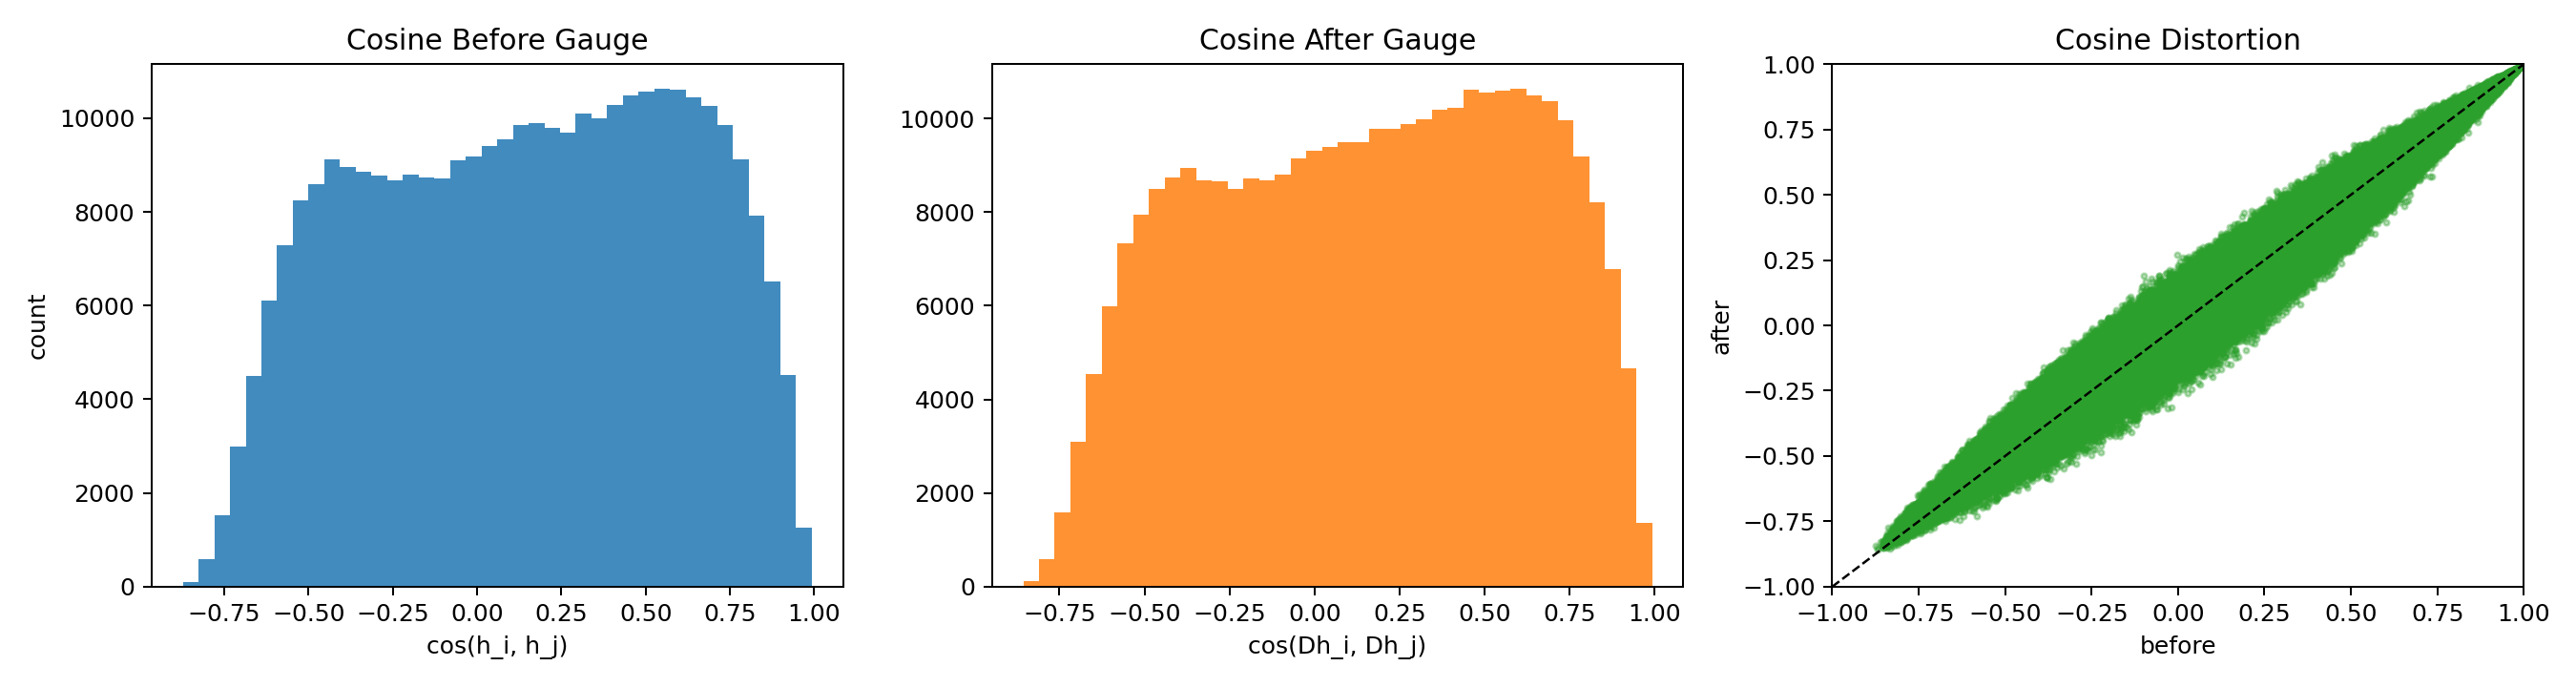
\includegraphics[width=\textwidth]{../experiments/figures/fig_cosine_distortion_cifar10.png}
\caption{CIFAR-10 cosine distortion under gauge transformation of
penultimate-layer features. Functional outputs are preserved after head
compensation, but cosine geometry shifts.}
\label{fig:cosine-distortion-cifar10}
\end{figure}

\begin{figure}[htbp]
\centering
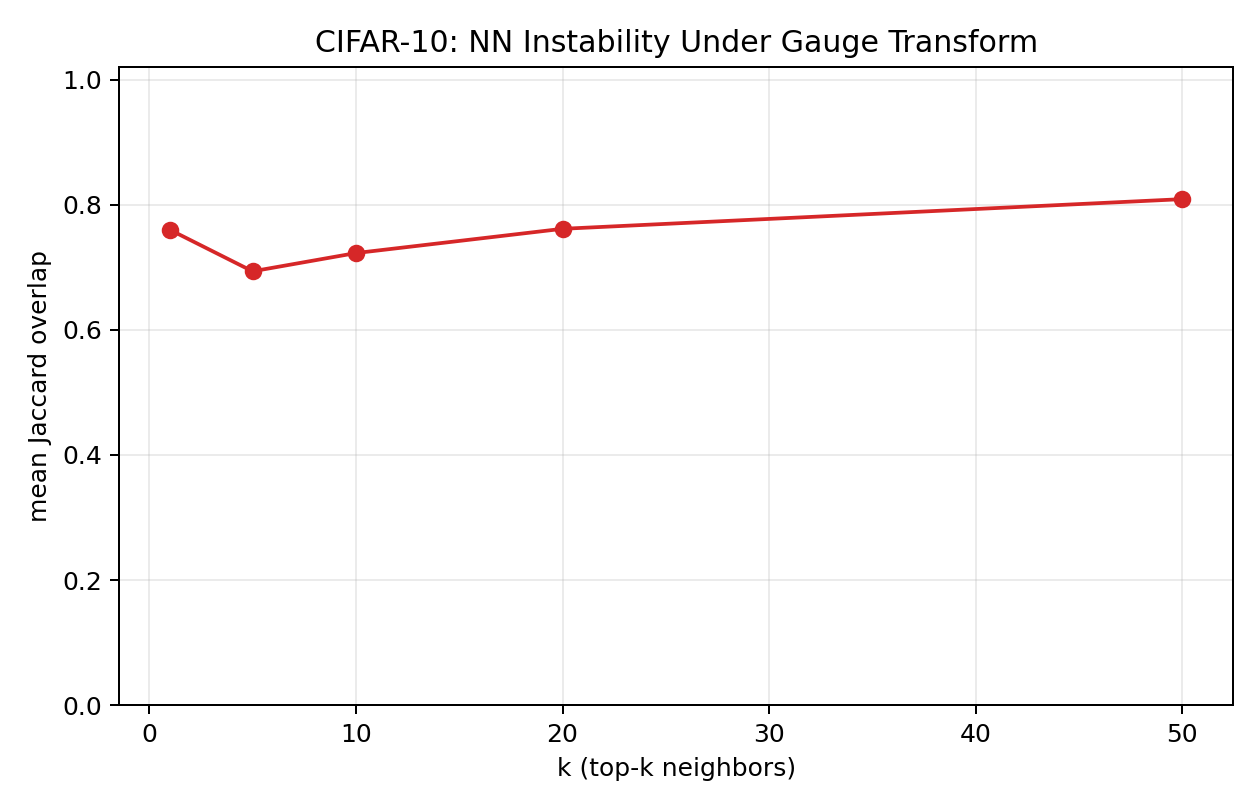
\includegraphics[width=0.75\textwidth]{../experiments/figures/fig_nn_instability_cifar10.png}
\caption{CIFAR-10 nearest-neighbor instability under gauge transformation.
Top-$k$ cosine neighborhoods are not invariant, mirroring the Digits
result in a more modern vision setting.}
\label{fig:nn-instability-cifar10}
\end{figure}

\begin{figure}[htbp]
\centering
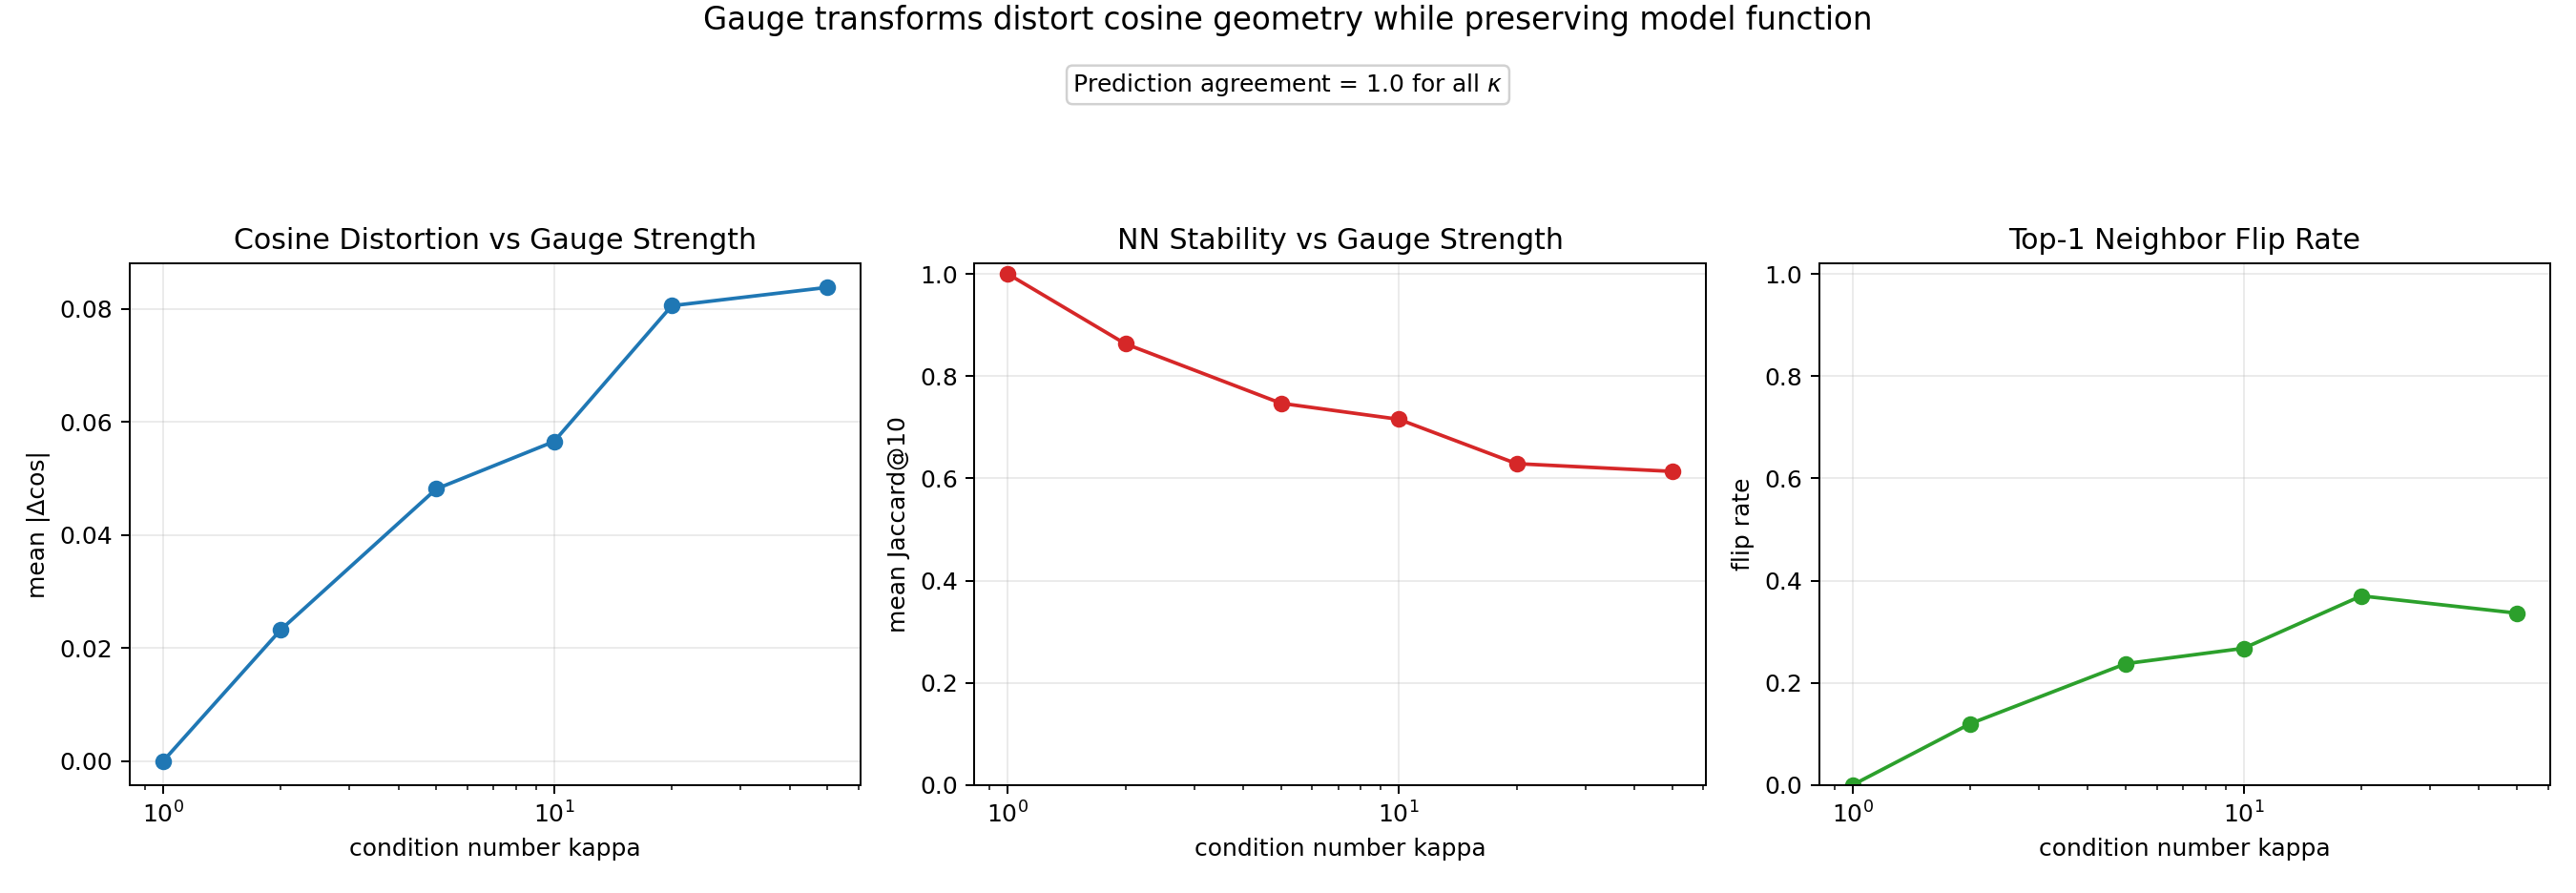
\includegraphics[width=\textwidth]{../experiments/figures/fig_cifar10_kappa_sweep.png}
\caption{CIFAR-10 controlled gauge-strength sweep.
As condition number $\kappa$ increases, mean cosine distortion grows,
nearest-neighbor overlap decreases, and top-1 neighbor flips increase,
while network outputs remain invariant after head compensation.}
\label{fig:cifar-kappa-sweep}
\end{figure}

\subsection{Whitening as Canonical Gauge Fixing}

For hidden representation matrix $H \in \mathbb{R}^{n\times d}$, we compute

\[
\Sigma = \frac{1}{n} H^\top H, \qquad D_{\mathrm{white}}=\Sigma^{-1/2},
\qquad H_{\mathrm{white}}=H D_{\mathrm{white}}.
\]

Before whitening, covariance eigenvalues were highly anisotropic
($\lambda_{\min}\approx 0.015$, $\lambda_{\max}\approx 36.58$).
After whitening, the eigenvalue spectrum collapsed to unity
(mean $|\lambda-1| \approx 6\times 10^{-6}$), as expected for isotropic
coordinates.

\begin{figure}[htbp]
\centering
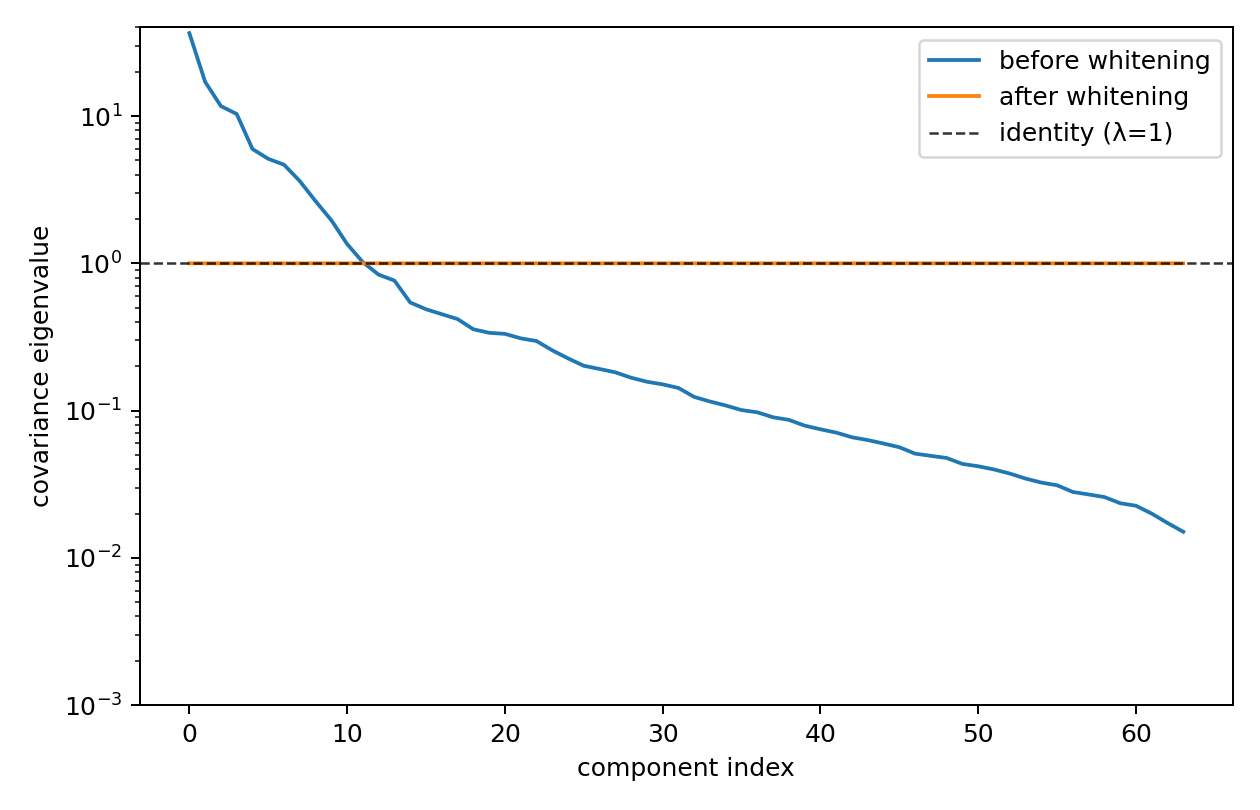
\includegraphics[width=0.8\textwidth]{../experiments/figures/fig_whitening_spectrum.png}
\caption{Covariance eigenvalue spectrum before and after whitening.
Whitening acts as a gauge fixing that normalizes anisotropic scaling in
representation space.}
\label{fig:covariance-spectrum-empirical}
\end{figure}

\begin{figure}[htbp]
\centering
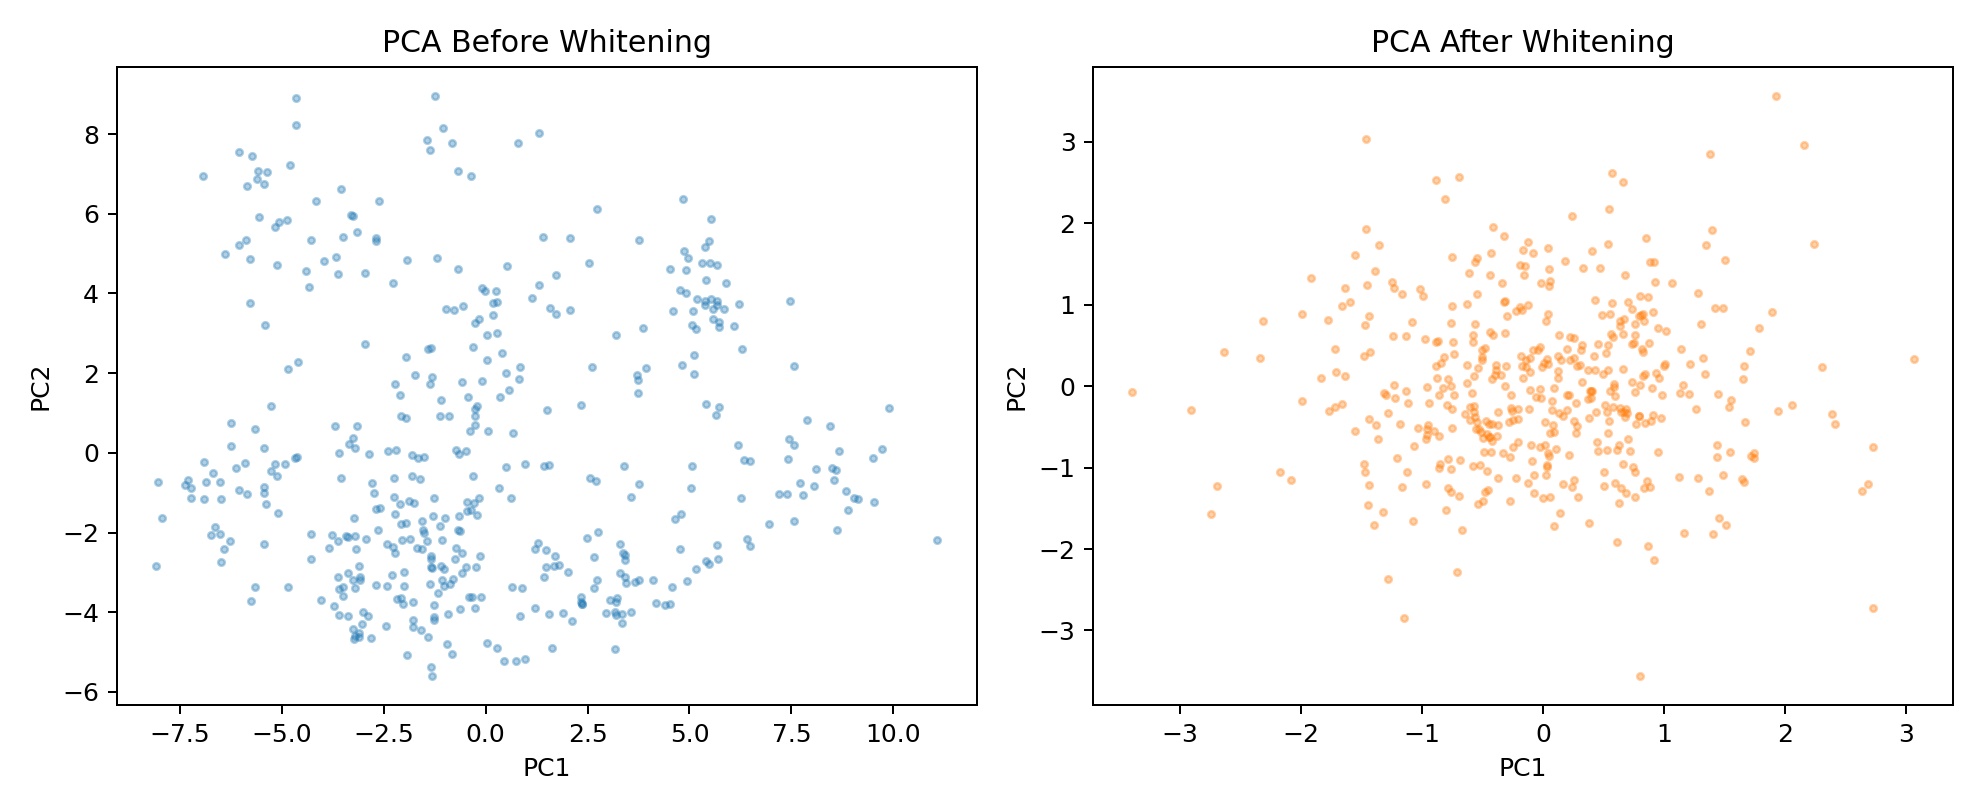
\includegraphics[width=\textwidth]{../experiments/figures/fig_whitening_effect.png}
\caption{PCA visualization of embeddings before and after whitening.
Whitening removes dominant anisotropic axes and yields a more isotropic
embedding cloud in transformed coordinates.}
\label{fig:whitening-effect-empirical}
\end{figure}

\subsection{Feature Geometry Stability Under Orthogonal Gauge Transforms}

As an additional check, we tested whether principal feature subspaces are
stable under a pure basis rotation.
Using an orthogonal matrix $Q \in O(d)$, we transformed hidden states as
$\tilde h = Q h$ and recomputed PCA.
If feature geometry is coordinate-dependent but information-preserving, then
the transformed principal directions should match the rotated original
directions up to basis ambiguity within each eigenspace.

Empirically, this behavior is observed.
For the top-$k$ principal subspaces, principal-angle cosines between the
expected rotated basis and the recomputed basis were numerically $1$,
and explained-variance ratios were unchanged up to numerical precision
(maximum difference $\approx 3\times 10^{-8}$).

\begin{figure}[htbp]
\centering
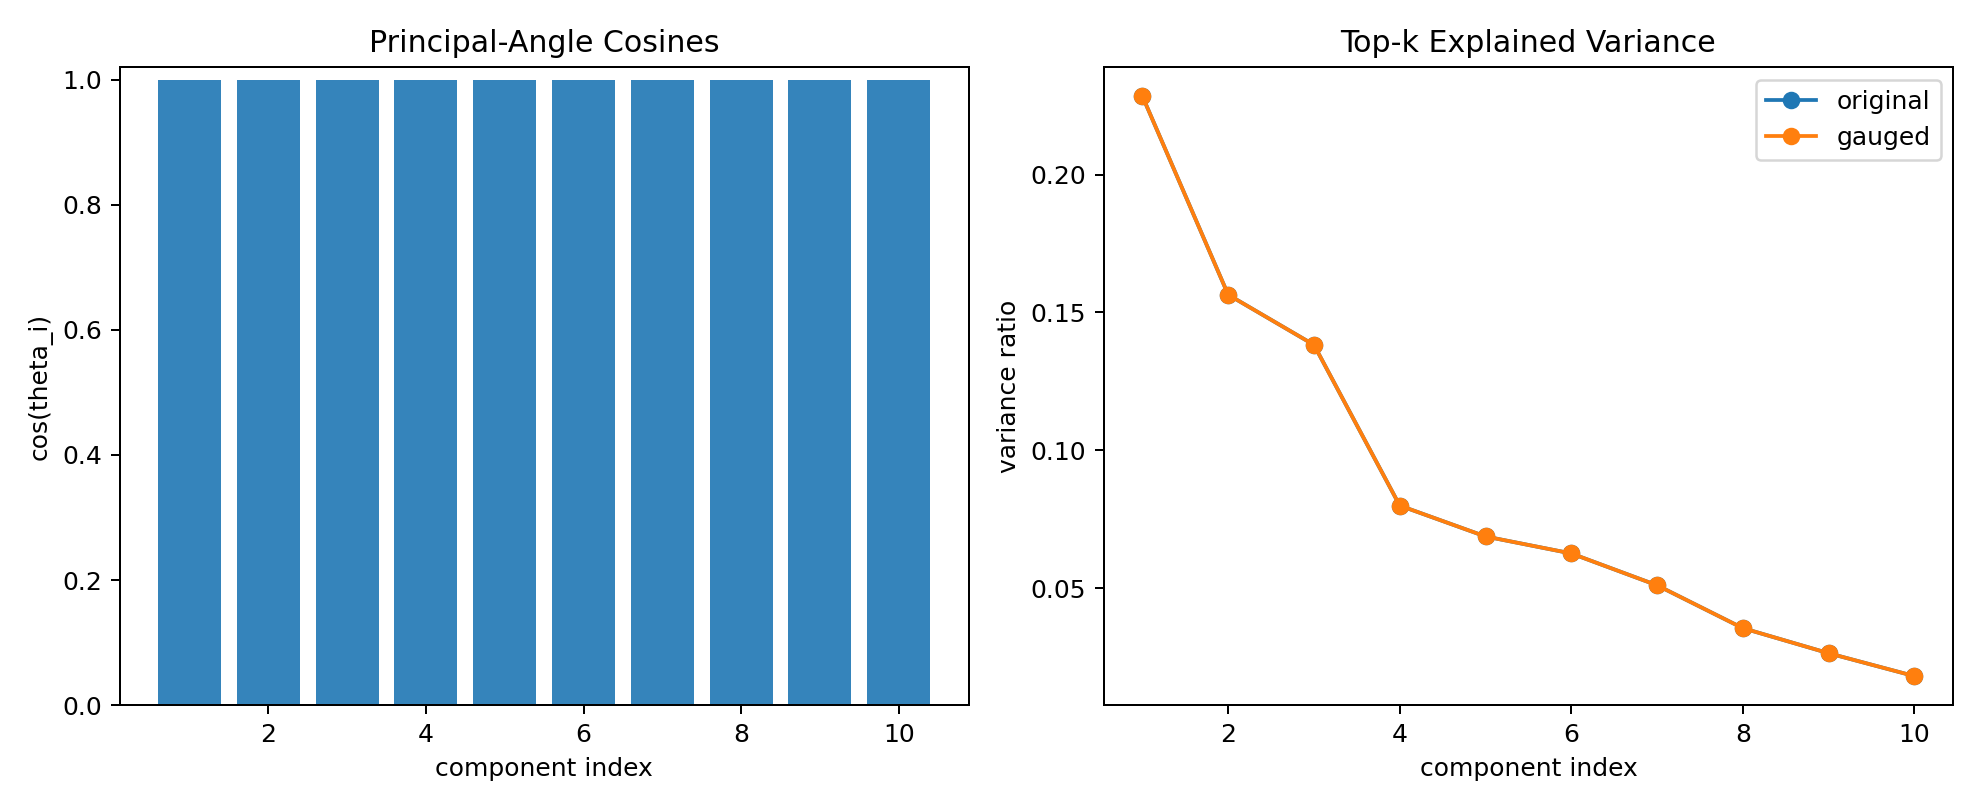
\includegraphics[width=\textwidth]{../experiments/figures/fig_feature_geometry_stability.png}
\caption{Feature geometry stability under an orthogonal gauge transform.
Left: principal-angle cosines between expected and observed transformed
PCA subspaces. Right: top-$k$ explained variance ratios before and after
transformation, showing near-perfect agreement.}
\label{fig:feature-geometry-stability}
\end{figure}

\section{Discussion}

The empirical results support the core geometric claim of this paper.
First, invertible linear transforms of representation space can be absorbed
by downstream weights, leaving model function unchanged to numerical
precision.
Second, cosine similarity is strongly gauge dependent: it can vary
substantially across equivalent coordinate systems.
Third, whitening provides a canonical coordinate choice that removes
second-order anisotropy and makes metric assumptions explicit.
Fourth, principal feature subspaces behave as expected under orthogonal
gauge changes: coordinates rotate while subspace content is preserved.

These findings clarify why cosine-based representation analyses can be
unstable across models, seeds, and training runs, even when predictive
behavior is similar.
They also motivate similarity measures and comparison procedures that are
explicitly invariant (or at least robust) to invertible transformations of
representation space.

\section{Conclusion}

Neural representations are not absolute coordinate objects; they are
defined up to gauge transformations in $GL(d)$.
This symmetry has direct empirical consequences:
model predictions can remain invariant while cosine geometry changes
substantially under invertible transforms.
Whitening can be interpreted as a practical gauge fixing that selects an
isotropic coordinate system.

Overall, representation analysis is most reliable when based on quantities
that are invariant under this gauge freedom or when metric assumptions are
made explicit and justified.

\bibliographystyle{plainnat}
\bibliography{refs_ml}

\end{document}
